% Chapter Intro

\chapter{Measurement of the CENNS with Cryogenic Bolometers in the RICOCHET experiment} % Main chapter title

\label{ChapterIntro} % Change X to a consecutive number; for referencing this chapter elsewhere, use \ref{ChapterX}

%----------------------------------------------------------------------------------------
%	BEGING CHAPTER
%----------------------------------------------------------------------------------------

\section{CE$\nu$NS and the new physics}

\subsection{Neutrino/core elastic coherent scattering}

A scattering phenomenon occurs when two particles interacts during a collision. A scattering is considered to be elastic when the energies of the two particles is conserved trough the collision, even though their momentum is not necessarily preserved. 
This work especially focuses on the elastic scattering between neutrinos and atomic nuclei. Event though the nucleus is an assembly of elementary particle, a coherent scattering occurs when the neutrino can interacts with the nucleus as a whole as if it was a uniform object.
When the scattering of a neutrino on a nucleus is coherent and elastic, it is defined as a Coherent Elastic Neutrino-Nucleus Scattering, shortened to CE$\nu$NS or CENNS.
This physical phenomenon, described by Freedman in 1973 within the framework of the standard model, was experimentally measured for the first time in august of 2017 by the collaboration COHERENT installed near the spallation source at the Oak Ridge National Laboratory in the United States.
Before getting to the heart of the matter, we can recall the various objects physical characteristics that will be discussed throughout this manuscript and present the scientific context of this work.
We will therefore discuss the atomic nuclei, the neutrinos, the CENNS equations and the various experiments aimed at measuring this very scattering process.


\subsection{The Atomic Nucleus}

Rutherford's experience with gold leaf in 1909 provided valuable information for the development of Bohr's atomic model in 1913. Rutherford understood that the electrically positively charged of an atom is concentrated in the middle of the atom. Indeed, knowing that the matter is electrically neutral and that an atom has electrons (charged negatively) there are necessarily positive charges "somewhere". Bohr then designed a atomic model for the hydrogen that reminds us of a planetary system. There would be the nucleus at center and the electrons around it, only allowed to be on specific circular orbitals.
Theoretical and experimental developments show us today that the electrons are not really on circular orbits but rather have a probability of presence described by combinations of spherical harmonics. Bohr's model for hydrogen is not fundamentally questioned and is still taught. Electrons are considered to orbit around the nucleus of positive charge. The latter can be either stable or unstable in the case of radioactive elements. 
This is an important fact, that an atom is not a fundamental object of modern physics: it is composed of nucleons (neutrons and protons), which are themselves composed of three quarks held together by to the strong nuclear interaction mediated by gluon. The size of an atom is of the order of of $\SI{0.1}{\nano\m} = \SI{1e-10}{\m}$ which five order of magnitude larger that the size of its nucleus $\SI{1}{\femto\m} = \SI{1e-15}{\m}$.


\subsection{The Neutrino}

The neutrino is one of the elementary particles of the Standard Model of Party Physics. Technically it is said to be an electrically neutral lepton. There are three flavors of neutrinos each associated with a lepton: the electronic neutrino $\nu_e$ is the equivalent of the electron $e^-$, the muonic neutrino $\nu_{\mu}$ for the muons $\mu^-$ and the tauic neutrino $\nu_{\tau}$ for the tau $\tau^-$.
The physicist Wolfgang Pauli was the first to postulate the existence of the neutrino in 1930. This new particle (at the time) helped to explain the continuous spectrum of the beta disintegration, which is a radioactive reaction in which a radionucleide emits an electron (or positron) and an (anti-)neutrino.
The experimental confirmation will be made in 1952 by Cowan and Queens based on an idea by Wang Ganchang (1942), the first two were awarded the Nobel Prize for physics in 1995 for this discovery.
A neutrino is only sensitive to the weak nuclear force and gravity. The later is negligible in particle physics but hold impact on the larger scale of cosmology. Due to the short range of the weak interaction \SI{e-18}{\m} the neutrino has a very low probability of interaction with matter, which is formalized in particle physics as a weak cross-section. To have an order of magnitude in mind we can show that out of 10 billion neutrinos of \SI{1}{\mega\eV} that cross the Earth, only 1 will interact with matter.
In the study of the CENNS process, no particular attention is brought on distinguishing  neutrinos from anti-neutrinos as well as different flavors. Indeed, this scattering process is insensitive to these differences. 


\subsection{CENNS and Standard Model}

It was in 1973 that Daniel Z. Freedman, a physicist currently at MIT, proposed the coherent elastic neutrino-nucleus scattering as a probe for weak interaction.
%[2]
 In its description based on the standard particle physics model still under development at the time (it will take its current form in the mid-1970s) Freedman expresses the evolution rate of the effective cross-section of the neutrino-nucleus interaction as a function of the recoil energy of the nucleus:
\begin{equation}
\label{eq:cenns-equation}
\frac{\mathrm{d} \sigma (E_{\nu}, E_R)}{\mathrm{d} E_R}
=
\frac{G_{f}^2}{4\pi}
Q_w^2  m_A
\left( 1 - \frac{m_A E_R}{2 E_{\nu}^2} \right)
F^2(E_r)
\end{equation}
This equation shows that the evolution of the effective cross-section noted $\sigma(E_{\nu} , \sigma{E_R} )$ depends on the neutrino energy $E_{\nu}$ and recoil energy $E_r$ of the nucleusas well as of the mass of the target nucleus $m_A$ and its composition $(N ,Z)$. Without going into the details of the theoretical calculations to obtain this expression, one can try to explain simply the different terms.

The Fermi coupling constant is measured experimentally by studying  the life time of the muon (inversely proportional to $G_f^2$).
%[3]
We can express this constant with the coupling constant of the weak interaction $g_W$ , the mass $m_W$ of the boson W, the speed of light $c$ and the reduced Planck constant $\hbar$ according to the equation:
\begin{equation}
G_f 
=
\frac{\sqrt{2}}{8}
\left( \frac{g_W}{m_W c^2} \right)^2
(\hbar c)^3
\sim \SI{1.17e-5}{\giga \eV^-2}
\end{equation}

The weak nuclear hypercharge $Q_w$ is given by:
\begin{equation}
Q_w = N - Z (1 - 4 \sin^2 \theta_w)
\end{equation}
It depends on the number of neutrons $N$ and protons $Z$ composing the nucleus. The term  $\theta_w$ is the mixing angle which is a parameter of the Weinberg-Salam theory of the electro-weak interaction (reunification of the theory of electromagnetism and weak interaction).
The value of $\sin^2 \theta_w$ is close to 0.24.
%[4] 
Thus, in practice, the hypercharge simplifies to $Q_w \simeq N$. As described later in this work, the measurement of the $\sin^2 \theta_w$ as a function of the transferred momentum would permit to probe for new physic in the electroweak sector.

The shape factor $F$ is a function of the recoil energy that characterizes the loss of coherence at high transferred momentum. It is worth 1 for low recoil energies, so it is often neglected in very low energy regimes, and decreases with the recoil energy $E_R$.

% (total)
The effective cross-section $\sigma$ associated with the CENNS is obtained by integrating the equation \ref{eq:cenns-equation} from $E_R = 0$ to $E_R^{max} = 2E_{\nu}^2 / (m_A + 2E_{\nu} )$, the maximum recoil energy of the nucleus accessible for a given neutrino energy $E_{\nu}$.
%[5]
Its expression is:
\begin{equation}
\sigma
\sim
\frac{G_f^2 N^2}{4\pi} E_{\nu}^2
\end{equation}
which is proportional to the square of the number of neutrons $N$ in the target nucleus and the energy of the neutrino thanks to the coherence of the interaction in case $m_N \gg E_{\nu}$.

The detection of CENNS is not done by directly measuring the cross-section of the particles that interact with the atomic nuclei of the detector. We measure the number of neutrinos having interacted with a nucleus according to the recoil energy of the latter. By doing this on a fairly wide range of recoil energy, we end up with what is called a energy spectrum of CENNS events. In this case, we will speak of CENNS spectrum, and of energy spectrum in the general case for different scattering processes. The expected differential CENNS event rate $R$ is calculated from the differential cross-section by convolving with the incoming neutrino flux $\Phi$:
\begin{equation}
\frac{\mathrm{d} R}{\mathrm{d} E_r}
=
\mathcal{N} \cdot
\int_{E_{\nu}^{min}}
\Phi(E_{\nu})
\cdot
\frac{\mathrm{d} \sigma (E_{\nu}, E_r) }{\mathrm{d} E_r} \mathrm{d} E_{\nu}
\end{equation}
In this equation, $\mathcal{N}$ represents the number of target nuclei per mass unit. The minimum energy of a neutrino to induce a nuclear recoil is given by the relation $E_{\nu}^{min}= \sqrt{m_N E_R /2}$.

A common representation of this type of interaction in particle physics is done with the help of Feynman diagrams. In this representation, the time flows from left to right and the distance between the particles is represented along the vertical axis. The mediator bosons are indicated with wavy lines. The figure \ref{fig:cenns-feynman} displays two Feynman diagram for the CENNS.
\begin{figure}
\centering
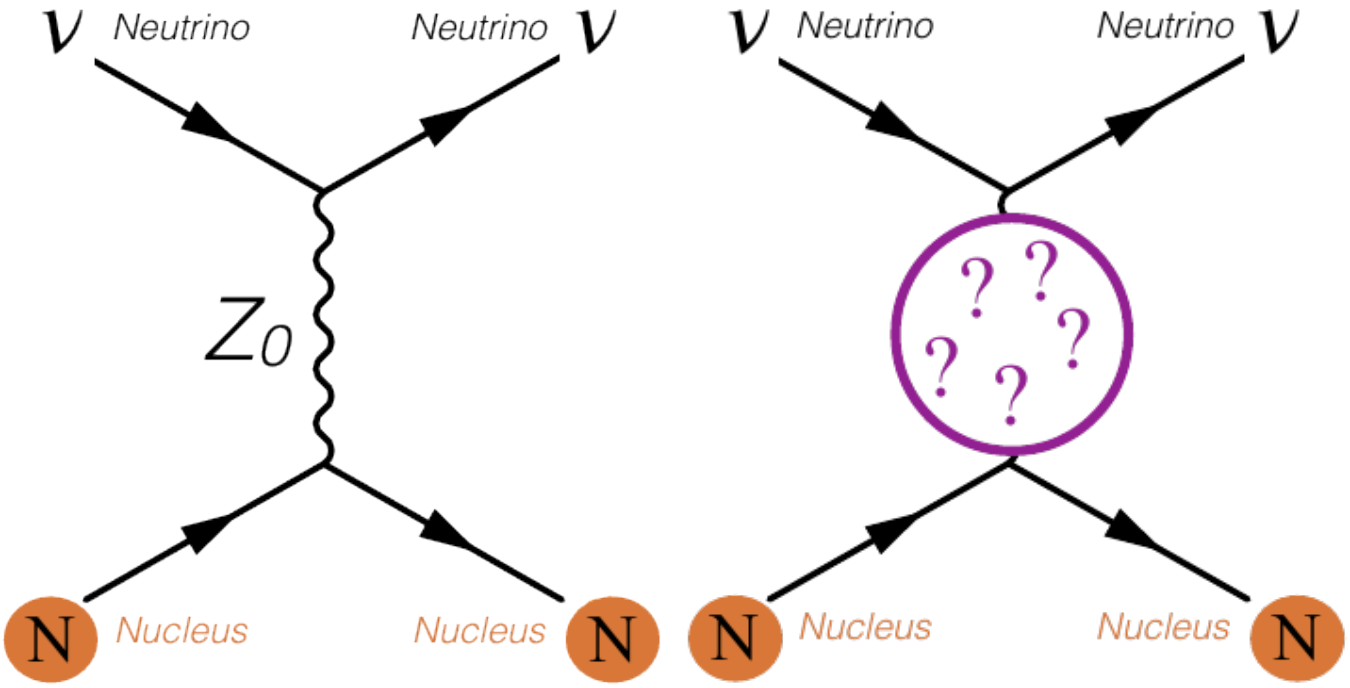
\includegraphics [scale=1]{Figures/Introduction/cenns_feynman.png}
\caption{Feynman diagram of the CEvNS. On the left in the case of the standard model. To the right the same process within the framework of alternative theories.}
\label{fig:cenns-feynman}
\end{figure}
The left diagram corresponds to the CENNS following the usual standard model by having the the $Z_0$ boson as the mediator of the weak interaction between the neutrino and the nucleus. The right diagram humbly presents the CENNS in the framework of alternative theories.


\subsection{First Detection of CE$\nu$NS}

The COHERENT collaboration was the first to observe experimentally and unambiguously the signature of the CENNS in August 2017.
%[6]
The technology used at that time was a \SI{14.6}{\kg} sodium-doped cesium iodide (\ce{CsI[Na]}) scintillator instrumented with photo-multipliers. The detector was located at a distance of \SI{19.3}{\m} from the neutrino source and had an energy detection threshold of \SI{4.5}{\kilo\eV}. The neutrino flux of average energy $E_{\nu} = \SI{30}{\mega\eV}$ used for this detection was produced with the so-called "pion-at-rest" method. It consists in taking advantage of the decay of positive pions, obtained after a controlled collision of a mercury atom with a proton, which leads to the production of neutrinos and anti-neutrinos. The proton source comes from the SNS (Spallation Neutron Source) located at the Oak Ridge National Laboratory in Oak Ridge, Tennessee (USA). 

Scientists in the collaboration have detected an excess of CENNS-related events, shown in Figure \ref{fig:coherent-result}, with a confidence of $6.7\sigma$ compatible at $1\sigma$ with the standard model. The uncertainty of the statistical study they estimate is \SI{16}{\percent}. This first detection of CENNS is a result which proves the existence of this phenomenon which has been considered for years by some as purely hypothetical. It has made it possible to constrain models of new physics 
%[6]
 but the current data do not allow to study the theories expected in the lower energies such as the existence of new mediating bosons.
%[7]
This requires a source of lower energy neutrinos.

\begin{figure}
\centering
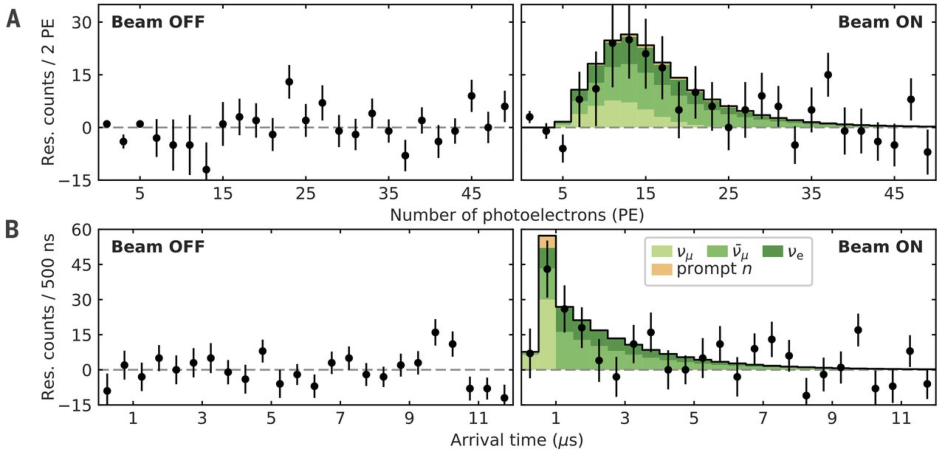
\includegraphics [scale=1]{Figures/Introduction/coherent_result.pdf}
\caption{Experimental result of the COHERENT experiment at the SNS demonstrating unambiguously the existence of the CENNS.}
\label{fig:coherent-result}
\end{figure}


\section{Search for New Low Energy Physics}

A number of theories diverge significantly from the prediction of the standard model at low energy. Among them we can mention in particular :
\begin{itemize}
	\item The existence of a new \ce{Z_0} mediator bosons,
	\item The existence of an abnormally high magnetic moment of the neutrino,
	\item The existence of non-standard interactions.
\end{itemize}

There is an important scientific stake in making these low energy measurements to provide additional elements in the understanding of fundamental interactions but also to provide additional constraints for a large number of neutrino research projects. A precise measurement of the CENNS would, for example, make it possible to constrain multiples theoretical models. 

However, to do new physics research with the CENNS process, the use of a suitable neutrino source is required. This source should have a known and adapted neutrino energy spectrum (typically $E_{\nu} \approx \SI{10}{\mega\eV}$). This will results in lowered recoil energies $E_R$ in the detector which should be be enhanced with higher sensitivities to the signal. This upgrade in detector performances can only be reached by diminishing the volume of the detectors resulting in a loss of exposure. As such, the new source should produce a very high flux of neutrinos as to counter the inevitable loss of detector mass and obtain an equivalent CENNS event rate.

Additionally, various technical and practical considerations are taken into account: possibility of interruption of the flow (or pulsed flow) for background rejection (as in the case of COHERENT for example), minimum accessible source/detector distance
%(the closer you are to the source, the closer you are to the detector) the greater the flow of neutrinos)
, ease of access and installation, regulations and availability of infrastructure.

\subsection{Neutrino Sources}

There are many sources of neutrinos because the radioactive decay processes that generate them are very common in nature. This subsection discusses some common neutrino sources and their characteristics regarding the search for the CENNS. Neutrinos out of experimental range such as those composing the neutrino diffuse background (the analogue of the neutrino diffuse cosmological background for neutrinos) will not be discussed. The resting pion method used by COHERENT will not be recalled as it has already been presented and is not a viable solution for the search for new low energy physics because of the too large energy of the emitted neutrinos.

\subsubsection{Solar Neutrinos}

Thermonuclear fusion reactions take place in the heart of stars. During these reactions, low energy neutrinos (a few \si{\mega\eV}) are emitted. They escape from their original star without great difficulty thanks to their low effective cross-section. The process responsible for about \SI{85}{\percent} of the neutrino emission of the Sun, is the fusion of two protons \ce{p} into a \ce{^2H} deuterium (heavy hydrogen) nucleus, an anti-electron \ce{e^+} (otherwise known as positron) and an electronic neutrino \ce{\nu_e}:
\begin{equation}
\ce{ p + p -> {}^2H + e^+ + $\nu$_e }
\end{equation}
For this specific reaction the energy of the emitted neutrinos is in the order of $\mathcal{O}(100)$ \si{kilo\eV}. It should be noted, however, that there are other reactions of a different nature producing neutrinos within the sun. The figure \ref{fig:solar-neutrino-spectrum} displays on the left, the simulated spectrum of the neutrino flux as seen from Earth associated with these different processes. Taking all energies together, from the Earth, the flux of solar neutrinos is of the order of \SI{7e10}{\cm^{-2} \s^{-1}} which is relatively small and makes the detection of solar neutrinos very difficult.

\begin{figure}
\begin{minipage}{0.48\textwidth}
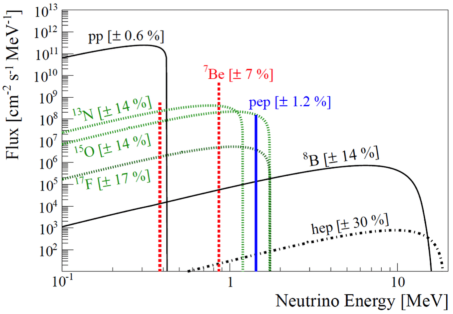
\includegraphics [scale=1]{Figures/Introduction/solar_neutrino_spectrum_simu.pdf}
\end{minipage}
\hfill
\begin{minipage}{0.48\textwidth}
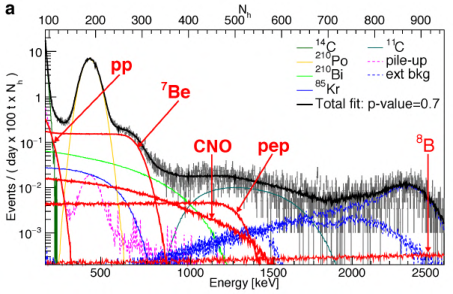
\includegraphics [scale=1]{Figures/Introduction/solar_neutrino_spectrum_exp.pdf}
\end{minipage}
\caption{Solar neutrino spectrum. On the left, simulated spectra of solar neutrinos seen from
the Earth associated with the different fusion reaction.
%[1]
On the right, solar neutrino spectrum and its components measured by the Borexino experiment at the Gran Sasso in Italy.}
\label{fig:solar-neutrino-spectrum}
\end{figure}

Despite this difficulty, large experiments, such as Borexino located in the underground laboratory of the Gran Sasso in Italy, are able to measure this solar neutrino spectrum as seen on the right subplot of figure \ref{fig:solar-neutrino-spectrum}. However, for a CENNS precision measurement experiment the sun is clearly not a relevant source because even if the energy of some neutrinos is low enough for probing new physics, it is not a relevant source of energy as the flux remains far too low and would require a huge volume (mass) of detector. Another negative point is that it is not possible to turn off the source to identify the background noise. Indeed, the solar neutrino flux is constant and crosses the Earth to reach the detector without difficulty.

\subsubsection{Terrestrial Neutrinos (geo-neutrinos)}

Our own planet, the Earth, emits neutrinos through natural radioactivity processes. Neutrinos resulting from these radioactive processes are numerous, it is estimated that the flow of neutrinos of origin geologic surface of the earth around \SI{1e6}{\cm^{-2} \s^{-1}}.
% [8]
This flux of geo-neutrinos is low and is coupled with a wide distribution in energy. Consequently, they are very difficult to detect because of the background of neutrinos from extraterrestrial and human origin. Nevertheless some experiments try to carry out geo-neutrino measurements for the information they would allow us to obtain on the Earth and in particular at the level of the Earth's core. The same large-scale experiment Borexino claims to have recently detected 53 events attributable to geo-neutrinos.
% [9]
For reasons similar to solar neutrinos, geo-neutrinos are not relevant in view of the current knowledge for CENNS precision measurement.

\subsubsection{Production from Human Activity}

Humans are capable of producing neutrinos in controlled physical processes. In particle accelerators, for example, it is not uncommon to produce neutrinos with energies of up to \SI{100}{\giga\eV}. The most intense man-made source of low-energy neutrinos are the the nuclear fission power plants. However, the main objective of these power generation plants is not the porduction of neutrinos, which consists in a very abundant by-product of the electricity production. The flow of neutrinos emitted by a standard nuclear power plant \SI{10}{\m} from the reactor is approximately equal to \SI{2e15}{\cm^{-2} \s^{-1}}, for an average neutrino energy of \SI{4}{\mega\eV}. Nuclear fission reactors offer a range of energy compatible with the research of new physics as envisioned by RICOCHET, the neutrino flux is among the most important and in addition to that it is possible to take advantage of unit outages to measure background noise. For this last point the subtraction background noise is not as optimal as with a pulsed source if the background noise is not stationary on the time scales represented by the combustion of a fuel rod but it is always an interesting plus to gain in measurement accuracy.


\subsection{Reactor Experiments}

The strong potential of nuclear power plants as sources of neutrinos has led a small number of CENNS experiments to be installed close to a reactor core around the world. The main experiments searching for the the CENNS near nuclear reactors are identified on the atlas displayed in figure \ref{fig:cenns-exp-atlas} and listed in the table \ref{tab:reactor-experiments} with their material used for their crystalline detector and their localization.

\begin{figure}
\centering
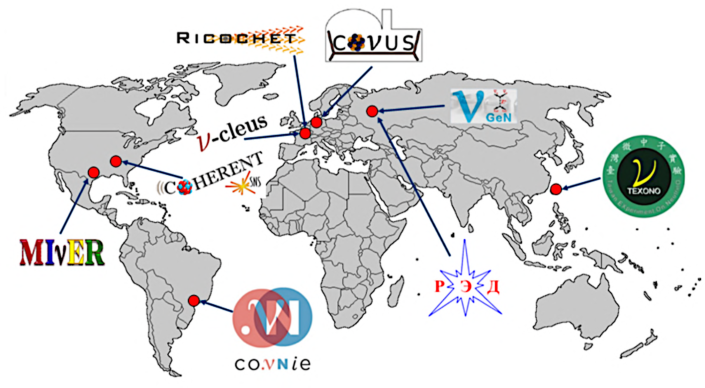
\includegraphics[scale=1]{Figures/Introduction/cenns_exp_atlas.pdf}
\caption{Main experiences of CEvNS in the world today (2020).
% Courtesy of Jules Colas
}
\label{fig:cenns-exp-atlas}
\end{figure}

\begin{table}[]
\centering
\begin{tabular}{c|c|c}
Experiment & (Detector Material) @ Location & Reference  \\ \hline \hline
NuGEN & 	(Ge) @ Kalinin Reactor (Russie) &	[10] \\
CONUS & 	(Ge) @ Brokdorf (Allemagne) &	[11] \\
TEXONO & 	(Ge) @ Kuo-Sheng Reactor (Taiwan) &	[12] \\
CONNIE & 	(Si) @ Angra Reactor (Brésil) &	[13] \\
RED100 & 	(Xe) @ Kalinin Reactor (Russie) &	[14] \\
MINER & 	(GeSi) @ Nuclear Science Center (USA) &	[15] \\
NU-CLEUS &	(\ce{CaWO_4}, \ce{Al_2O_3} ) @ Chooz (France) &	[16] \\
RICOCHET & 	(Ge, Zn, Al, (Si)) @ ILL (France) &	[17] \\
\end{tabular}
\caption{Presentation of CENNS experiments associated with a nuclear reactor: materials used for detection @ localization. In red are represented the cryogenic experiments with a very low detection threshold for the research of new physics. The RICOCHET experiment is the only one to propose a detector capable of discriminating between nuclear and electronic recoils.}
\label{tab:reactor-experiments}
\end{table}

The CENNS experiments near a reactor would allow the estimation the Weinberg angle $\theta_w$ at low energies. Figure \ref{fig:weinberg-angle} shows the prediction of the standard model (blue line) for this parameter and the zone of the parameter space accessible by the CENNS experiments (green zone) which still remains largely unexplored. The estimation of this parameter with different physical processes is also very important to identify incompatibilities and allow the scientific community to go beyond the current theoretical model.

\begin{figure}
\centering
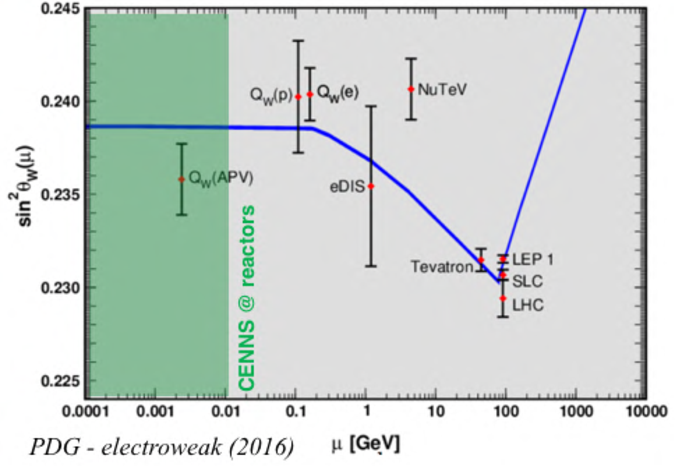
\includegraphics[scale=1]{Figures/Introduction/weinberg_angle.pdf}
\caption{Measurements of the Weinberg angle as a function of the impulse (or transferred moment). The blue curve is the prediction of the standard model for different processes and experiments. The green area shows the area accessible with a precision measurement of the CENNS spectrum near a nuclear reactor.}
\label{fig:weinberg-angle}
\end{figure}

In view of the number of CENNS experiments, we can expect this precision measurement within a few years. What is uncertain is whether this scientific result will deviate from the standard model at low-energy scale or confirm this theory. The "cooperation" at work between all these collaborations and with dark matter experiments such as EDELWEISS favors rapid developments and technological improvements.


\subsection{RICOCHET}

RICOCHET is a CENNS experiment led by the members of the MANOIR team at the \textit{Institut de Physique des deux Infinis} (IP2I) of Lyon, which brings together some fifty researchers, technicians and engineers through various laboratories and universities in France, Russia and the United States. RICOCHET aims at measuring the CENNS spectrum with a statistical accuracy of \SI{1}{\percent} after one year of taking data. With this objective, the detection CENNS with low energy neutrinos (a few \si{\mega\eV}) with an accuracy of at least $5\sigma$, like the COHERENT experiment, will be reached within a week of operation. 
It should be noted that the targeted accuracy is far superior to that obtained by COHERENT. To achieve these scientific objectives the RICOCHET device is composed of a cryogenic system, a shielding to limit sources of unwanted noise and the CRYOCUBE detector. It will be installed in 2022 at the Laue Institute Langevin (ILL) in Grenoble, France. The ILL hosts a \SI{58}{\mega\watt} fission research nuclear reactor. A numerical modeling of RICOCHET at ILL and the implementation scheme near the reactor core are presented in figure \ref{fig:ricochet-ill-site}.

\begin{figure}
\centering
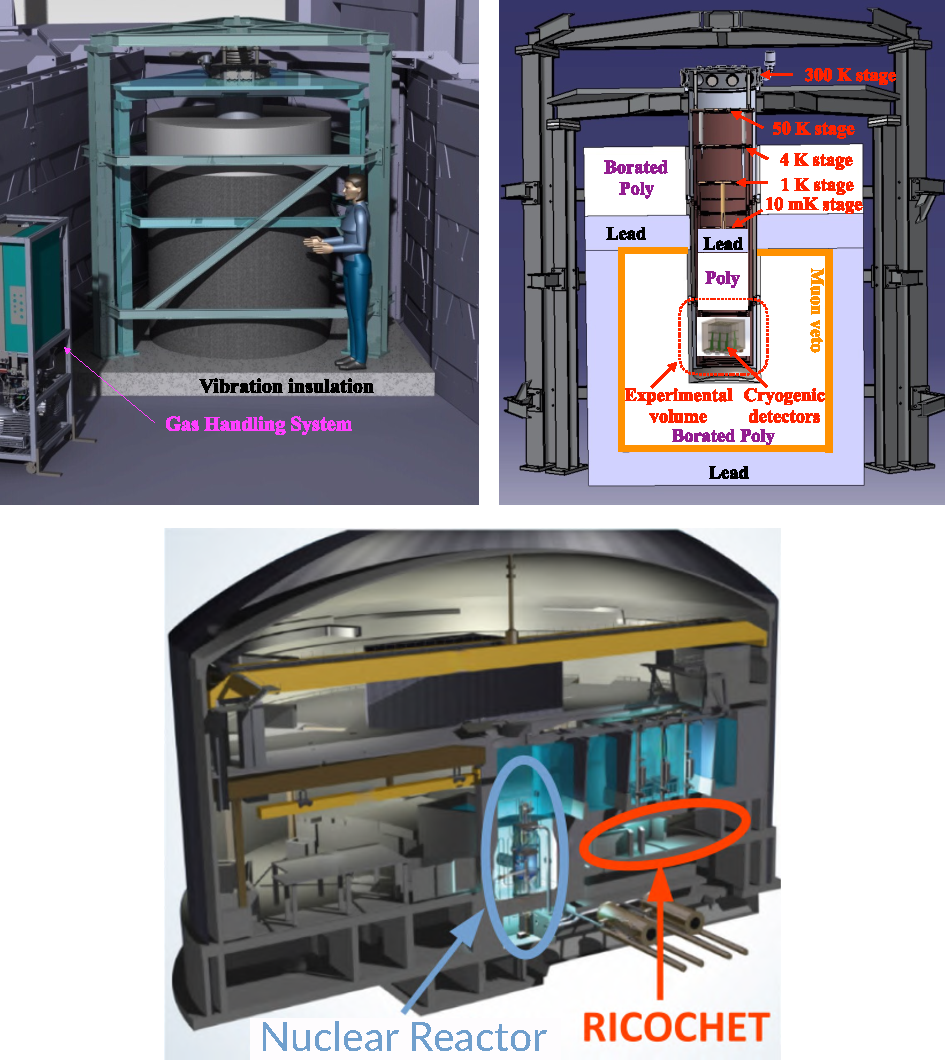
\includegraphics[scale=1]{Figures/Introduction/ricochet_ill_site.pdf}
\caption{On the top left Installation of RICOCHET at ILL, 3D modeling. On the top right, View in
cryostat cut. At the bottom, location of the RICOCHET cryostat within the ILL nuclear reactor. The water pool above the location of RICOCHET provides protection against cosmic particles.}
\label{fig:ricochet-ill-site}
\end{figure}

The CRYOCUBE detector will be at only \SI{8}{\m} from the core of the nuclear reactor with a power of \SI{58}{\mega\watt} which will produce a neutrino flux of \SI{e12}{\cm^{-2} \s^{-1}}. The CRYOCUBE will be cool down close to the absolute zero at cryogenic temperatures comprised between 5 and \SI{20}{\milli\kelvin}, in order to be able to measure minute temperature rises caused by the neutrinos during their interaction with the nuclei that make up the detector's target material.

%The operation of the CRYOCUBE detector will be detailed later. But it is necessary to know that 
The cryogenic detector load will be protected from external radiation by a thick layer of lead and borated poly-ethylene shielding weighting more than 15 tons and an active cosmic particle rejection device designated as "veto muon". The objective of this shielding strategy is prevent as much as possible any unwanted diffusion processes in the experimental data which would increase the signal-to-noise ratio and significantly hurt the chances of detecting signs of new physics.

The incident neutrino flux on the location of the CRYOCUBE at the ILL site was estimated and
the Manoir team has precisely simulated the expected CENNS spectrum according to different theoretical models considered and taking into account the different background noises. On the left subplot of figure \ref{fig:cenns-new-physics}, we see the prediction of the standard model (in blue) and the assumed effect of two alternative theories: the existence of an abnormally high neutrino moment (violet, fine dotted line) or of a new particular Z' boson (violet, dashed line). The background noise, of electronic or nuclear origin, is represented in grey and is both almost uniform in the energy range considered.

This numerical simulation allows to define the specifications of RICOCHET so that the CENNS spectrum is measured specifically in the region of interest for the new physics. From the spectra associated with two exotic physics scenario in figure \ref{fig:cenns-new-physics}, we see that we need a low enough detection threshold in recoil energy. Otherwise, we will not be able to see the deviations from the standard model or even the CENNS itself.

\begin{figure}
\centering
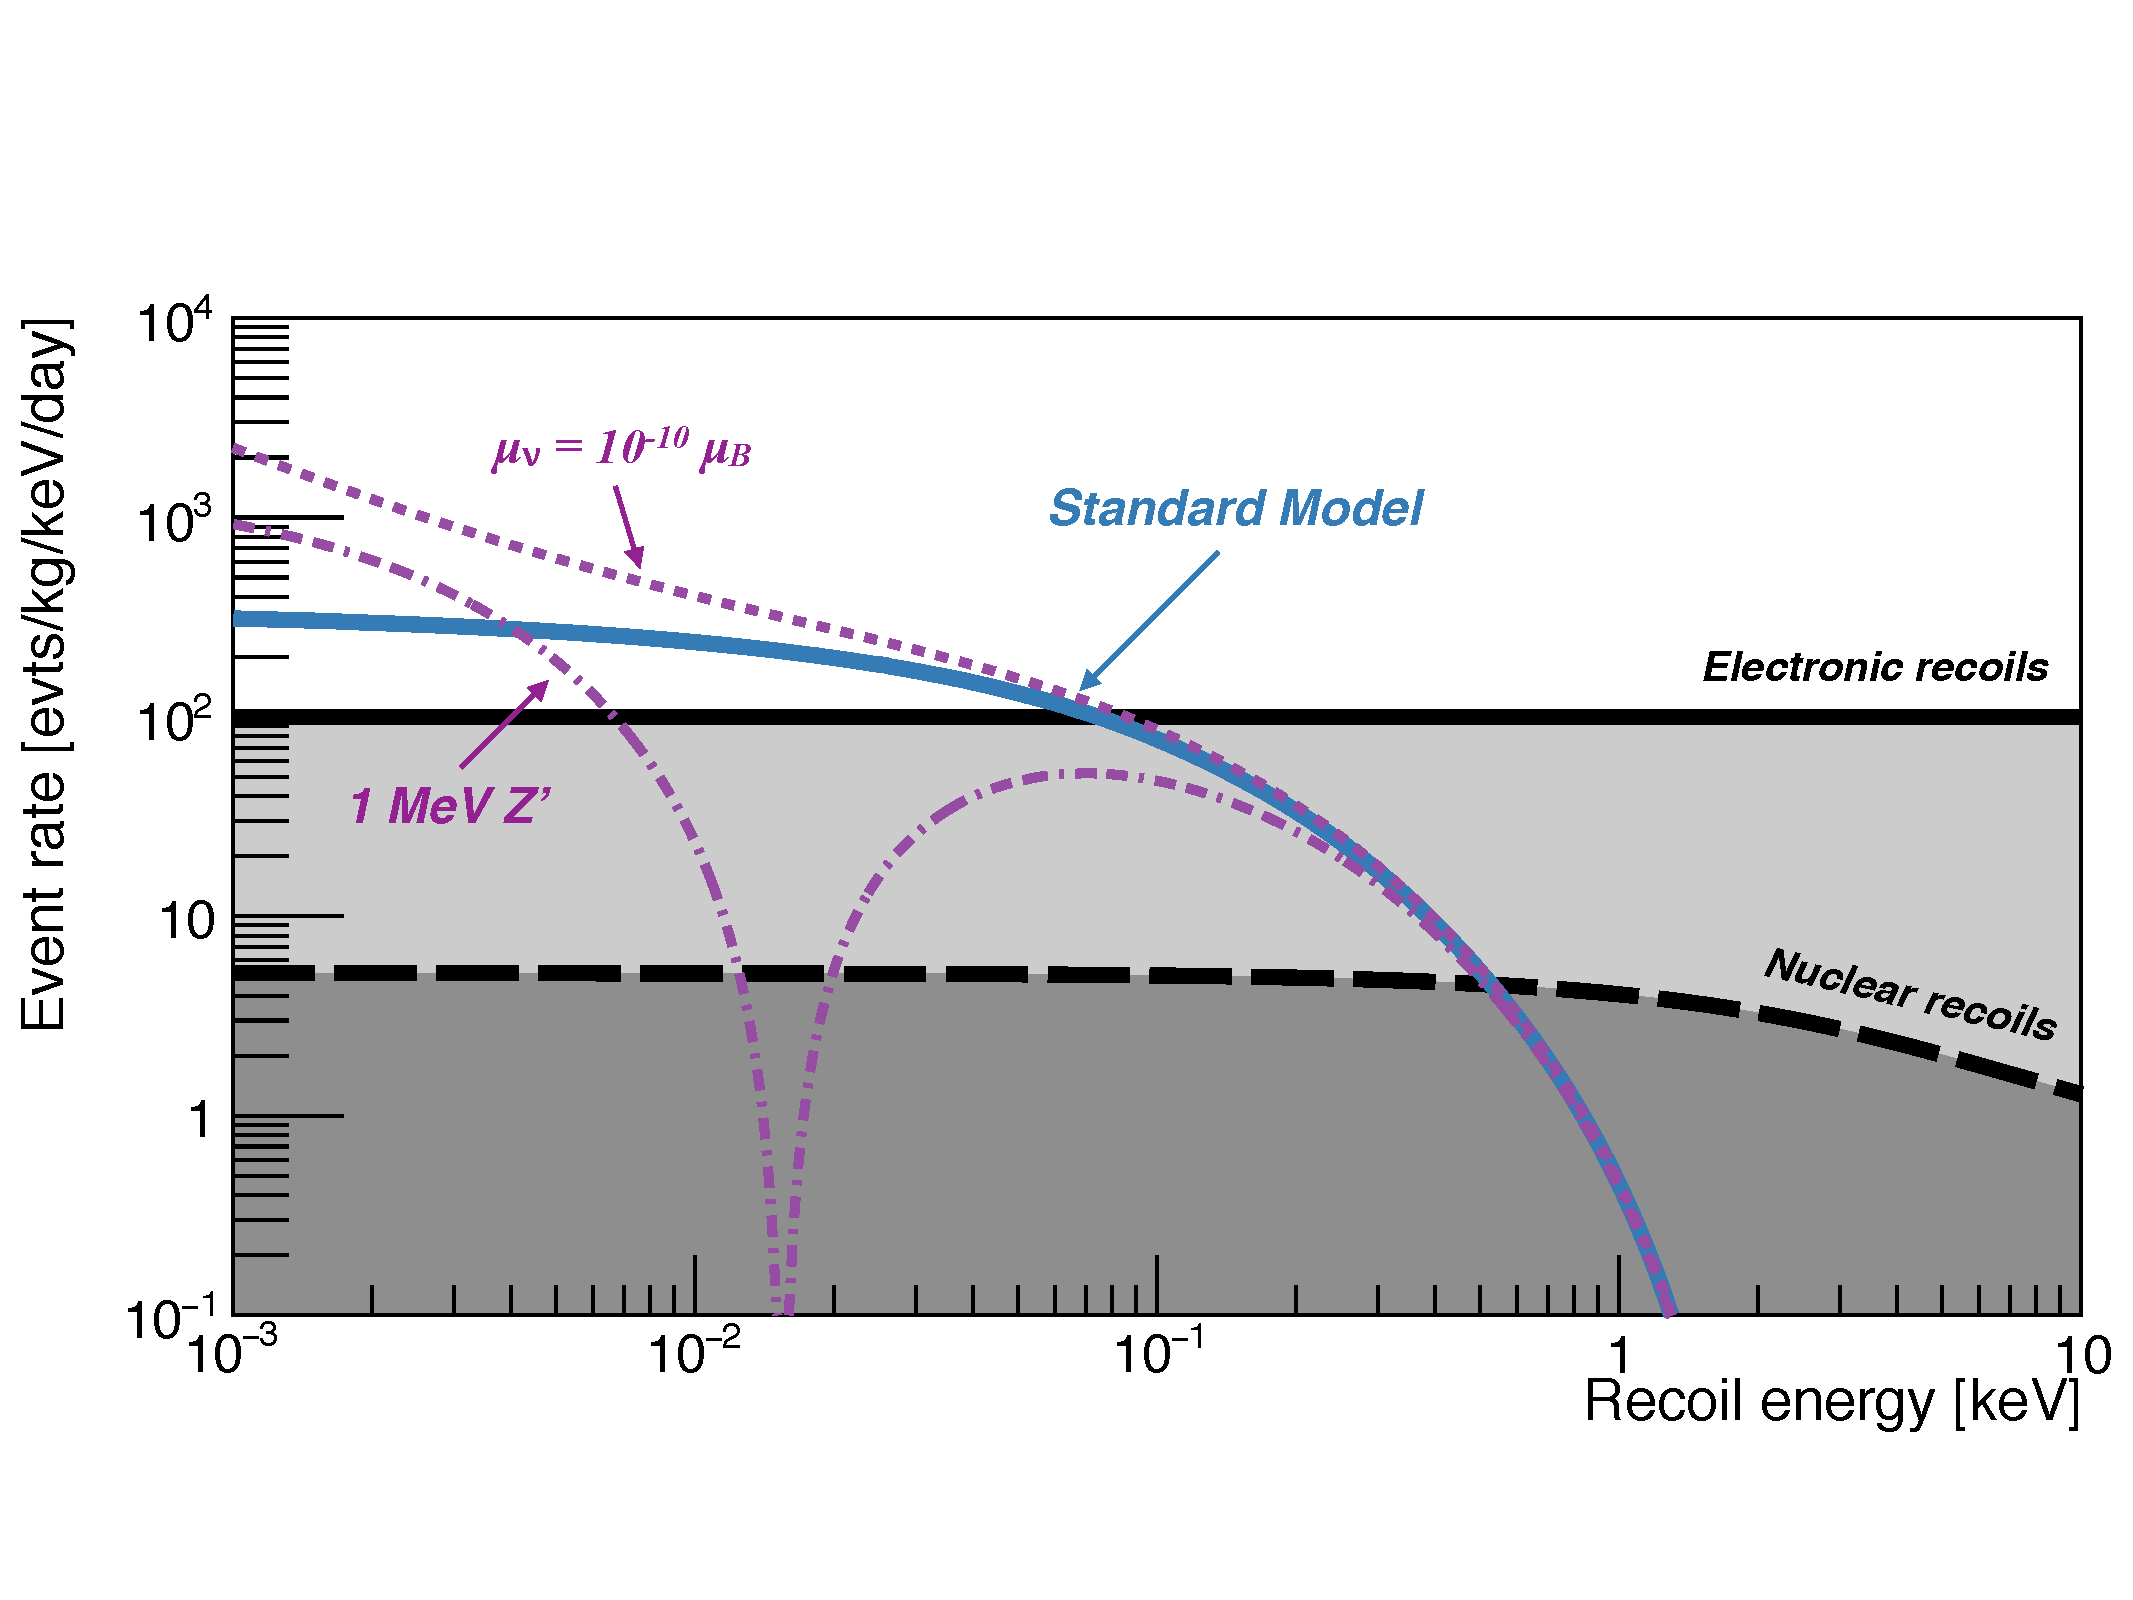
\includegraphics[width=0.7\textwidth]{Figures/Introduction/cenns_spectrum_ill.pdf}
\caption{On the left, Simulation of the background noise on the CENNS spectrum for RICOCHET at the ILL. The radioactive background noise is represented as its two components inducing electronic recoils in light grey and inducing nuclear recoils in dark gray.}
\label{fig:cenns-new-physics}
\end{figure}

We can notice that the spectrum is given in \si{events \per \kilo\eV \per \kg \per \day} and therefore to have a sufficient statistic it is necessary to find an interesting ratio of detector mass over data acquisition time.
Indeed having an ultra massive detector represents a real technical challenge. One can quote for example the dark matter research experiment XENON1T which uses a detector whose total mass is greater than one ton and its version in development XENONnT which aims to go even further in terms of mass. This detector technology, based on a liquefied noble gas, is not the most efficient for the CENNS but above all requires a large experimental volume that is difficult to obtain near a nuclear reactor.
Other technologies such as super-K or Borexino experiments would be theoretically possible but the experimental volume would remain an impossible constraint to reconcile with the proximity to the nuclear reactor.
The opposite approach consists in taking a low detector mass, which easier to install, operate, analyze and protect from external background noise, and collecting experimental data for a long time. In theory there would be no problem to this, but in practice the non-stationarity of the noise, the volume of the data, the time to analyze this data and the time of experience (mobilization of human resources, technical, infrastructure, ...) make the task very difficult. There is therefore a compromise to be made between the mass of the detector and the desired duration of data acquisition for a given number of CENNS events.

The exposure of the detector, its mass multiplied by the experiment time) in \si{\kg \day}, is not the only parameter to be considered, it is necessary to have sufficient sensitivity to measure the minute variations in temperature generated by the interaction of a neutrino with matter and to be able to differentiate between nuclear and electronic recoils in order to increase the signal-to-noise ratio (as suggested by numerical simulation). 

To carry out this identification of neutrino recoils, one way to do this is to measure the temperature increase induced by a deposit of energy while measuring the electron-hole pairs created in the semiconductor material that serves as a target for coherent elastic scattering. 
This double energy measurement is described later in the section \ref{sec:detector-principle}.

Specifically, a detector with the following characteristics would be required:
\begin{itemize}
	\item Detection threshold / energy resolution: $E_R \sim \SI{50}{\eV}$ / $\sigma(E_R) \sim \SI{10}{\eV}$
	\item Ability to discriminate between electronic and nuclear recoil with thermometer + electrodes for electronic noise rejection with semiconductor material 
	\item Mass of the detector: $m_d \sim \SI{1}{\kg}$ with a flux of \SI{e12}{\cm^{-2} \s^{-1}} to have about ten of CENNS events per day
\end{itemize}

To meet these specifications, the members of the RICOCHET collaboration are developing an innovative detector called CRYOCUBE which is presented in the figure \ref{fig:cryocube}. It will be composed of 27 germanium crystals of \SI{38}{\g} equipped with a heat measurement channel and an ionization measurement channel for discrimination purpose.
%The energy threshold of \SI{50}{\eV} on the heat channel has already been demonstrated with the RED20 prototype.

\begin{figure}
\centering
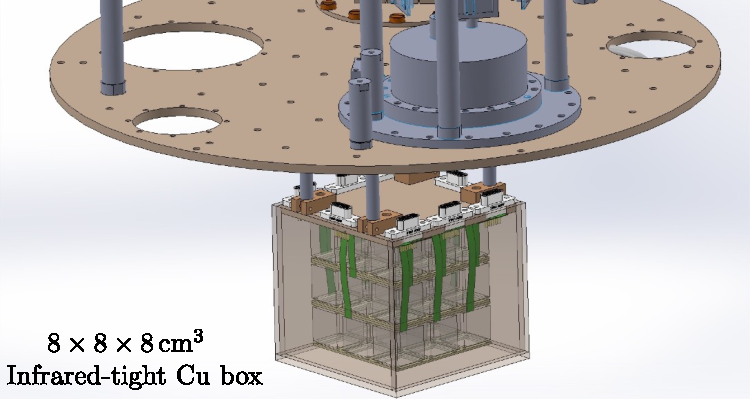
\includegraphics[scale=1]{Figures/Introduction/cryocube.pdf}
\caption{3D model of the CRYOCUBE installed at the coldest stage of its cryostat. We can see by transparency the 27 germanium crystals of 38g electrically connected to the systems of acquisition by the green cables.}
\label{fig:cryocube}
\end{figure}





%RICOCHET is a relatively large scientific experiment that requires good project management. The implementation of the CRYOCUBE technology, through the joint development program RICOCHET and EDELWEISS on RED detectors is a very expensive step. For information, each 30g germanium crystal costs about ten thousand euros because of the requirements of purity and geometry (polishing, ...). One understands the need to deepen the approach and optimization on single crystal detectors before building the final CRYOCUBE. The CRYOCUBE project is supported by an ERC starting grant awarded to Julien Billard, IP2I researcher. The cryostat to host the CRYOCUBE is custom-built by the French company CryoConcept and financed by our Russian collaborators to the tune of five hundred thousand euros, to which must be added shielding, electronics, computer systems and human resources costs. Excluding human resources, RICOCHET's installation at ILL is estimated at more than three million euros (all funding combined: ANR, ERC, laboratories, ...).
%


%\section{Theoretical Objectives}
%
%The R\&D team of the MANOIR group is developing cryogenic bolometers for the search of low energy chargeless particles. Its work contributes to the EDELWEISS and the RICOCHET experiments.
%
%The EDELWEISS is a direct dark matter search experiment. The dark matter problem emerges from discrepancies between cosmological observations and theoretical expectations (galaxies spinning faster than expected from their luminous masses for example). Even though there is a lot of theories (MACHO, modified gravitation, etc...) which could explain these differences, the favorite is the existence of a Weakly Interacting Massive Particle (WIMP). This particle is non relativist, chargeless and rarely interact with ordinary matter. According to cosmological constraints, WIMP particles forms a halo/cloud comprising our galaxy, meaning that this particles are present and could be detected on Earth.
%
%The RICOCHET is a neutrino experiment for the precise measurement of the Coherent Elastic Neutrino-Nucleus Scattering (CENNS). Predicted in the 70s, this process was only discovered in 2017 thanks to modern technology. The study of this process at low energy level could unravel new physics but this calls for very sensitive neutrino detectors. Coincidentally, dark matter detectors are well-adapted to the challenges of the CENNS measurement although few adjustments and a proximity to a neutrino source (like a nuclear reactor) are needed.
%
%\section*{Introduction}
%
%The problem of dark matter has been motivating many physicists in the fields of cosmology, astrophysics and particle physics for several decades. Various cosmological observations have indeed proved the presence of non-visible mass in the universe, and thus created one of the major challenges of modern physics. The great emulation present in this field of study has given birth to many scientific collaborations, and with them, many experiments for the research of dark matter.
%
%It is in this scientific context that I carried out my second year Master's internship within the Manor Group of the IPNL whose work is part of the EDELWEISS collaboration. She is working on a direct detection experiment located in the Laboratoire Souterrain de Modane under the Fréjus tunnel. Recently reconverted in the search for light dark matter, the collaboration is relaunching a research and development campaign to obtain detectors with low energy detection thresholds.
%
%This report describes the development work on cryogenic detectors that I carried out during 4 months. I had the opportunity to perform experimental data acquisition on the IPNL R\&D crysotat, to develop theoretical tools for detector modeling and to compare the modeling with the experimental measurement.
%The first part of the report is devoted to a reminder of the dark matter problem, and to the description of the detection principle used in the detectors of the EDELWEISS experiment. In a second part, the two detectors studied (RED1 and RED10) are presented and an electro-thermal model is built. The third part gathers the different experimental results. There is first a characterization of the electronics with the RED1 detector, then a thermal characterization of RED10 with comparison to the electro-thermal model. We will finish with the preliminary optimization results using all the results presented in this report.
%
%\section*{Introduction}
%
%
%\section{The detection of light dark matter within EDELWEISS}
%
%\subsection{Dark matter evidence}
%
%There is evidence of the existence of dark matter at several scales. At the cosmological scale, for example, it is the latest measurements from the PLANCK \cite{planck} collaboration that provide an energy-matter composition of the universe. This would be composed of only $4\%$ of baryonic matter while dark matter would represent $26.1\%$. On a rather local scale, we have the work of Vera Rubin who has highlighted this dark matter by studying the distribution of velocities within spiral galaxies. A curve of the velocity of the stars as a function of their distance from the galactic center is presented in figure \ref{galaxy}.
%
%\begin{figure}[!ht]
%\begin{center}
%\includegraphics [scale=1]{Images/curve_rot.pdf}
%\end{center}
%\caption{The velocities of the stars in the spiral galaxy are represented according to their distance from the galactic center. The measured velocity curve (in black) is compared to the one simulated (in green) from the measured luminous mass. The red curve corresponds to the velocity curve of the dark matter halo potential. Figure from \cite{spiral}.}.
%\label{galaxy}.
%\end{figure}
%
%The experimental measurements (in black) are compared with the velocity curve calculated from the luminous mass of the galaxy (in red). The velocity curve does not decrease with the distance contrary to the prediction, but remains constant. To explain this, it is necessary to add to the model the presence of a massive and non-luminous halo encompassing the luminous matter (in green), this would be the famous dark matter.
%
%
%\subsection{Introduction of the WIMP candidate}
%
%Several hypotheses about dark matter have already been put forward. The idea that dark matter can be made of baryonic objects such as black holes or brown dwarfs is discarded. Indeed, the MACHO (MAssive Compact Halo Object) and Eros experiments have shown that such objects could not explain more than $10%$ of the observed dark matter contribution. We therefore converge towards a model where dark matter is made of particles. Another hypothesis proposing neutrinos as a candidate comes up against the scenario of formation of the structures of the universe. This so-called "bottom-up" scenario, where small structures are precursors to large ones, indicates the non-relativity of dark matter particles, called cold dark matter.
% 
%Numerous observations have allowed to draw up an inventory of the constraints that dark matter must respect. The most likely candidate for dark matter, respecting at best these constraints, is the WIMP (Weakly Massive Interacting Particle). It is a particle:
%\begin{itemize}
%\item Massive and non-relativistic, with a mass of between $1$Gev and $1$TeV,
%\item Neutral electrical load, therefore not subject to electromagnetic interaction,
%\item neutral in color, therefore not subject to strong interaction,
%\item interacting by low interaction with a very low effective section,
%\item detectable from a terrestrial laboratory, its flux is estimated at about $10^5$WIMPs/cm${}^2$/s.
%\end{itemize}
%
%\subsection{Dark matter detection methods}
%
%The search for dark matter is therefore equivalent to searching for WIMPs. There are three detection methods illustrated in figure \ref{3way} :
%\begin{itemize}
%\item Indirect detection is equivalent to observing the possible annihilation product of two dark matter particles that would then produce observable standard model particles, such as neutrinos, gamma radiation, or antimatter.
%\item Production is equivalent to studying Standard Model particle collision processes in collider-type experiments such as the Large Hadron Collider. A loss of energy in the energy balance could be explained by the production of dark matter that would escape the detectors.
%\item Direct detection is the study of the elastic collision between a WIMP and a target nucleus. The measurement of the recoil energy deposited by the WIMP allows to deduce its mass as well as the effective cross-section of the interaction process.
%\end{itemize}
%
%\begin{figure}[!ht]
%\begin{minipage}{0.49\textwidth}
%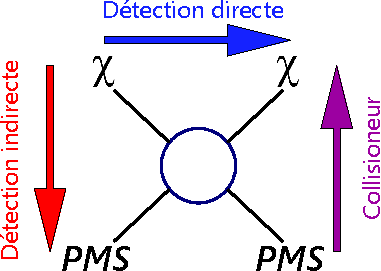
\includegraphics [width=\textwidth]{Images/direct_detection.pdf}
%\end{minipage}
%\hfill
%\vrule{}
%\hfill
%\begin{minipage}{0.40\textwidth}
%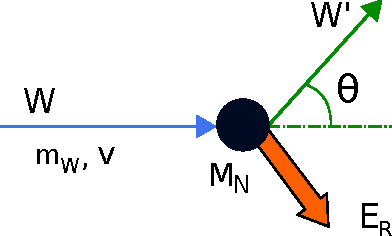
\includegraphics [width=\textwidth]{Images/wimp_diff.pdf}
%\end{minipage}
%\hfill
%\caption{(left) Graphical representation of the different methods of dark matter detection. $\chi$ designates a dark matter particle and $PMS$ designates a standard model particle. \\
%(right) Representative scheme of the elastic collision of a WIMP, noted \textbf{W}, on a kernel, \textbf{N}. The WIMP then transfers a recoil energy $E_R$ to the kernel.}
%\label{3way}
%\end{figure}
%
%These three detection channels are complementary. Indeed, each method observes the interaction diagram of figure \ref{3way} in a different way. As the analysis of the experimental results depends on the model used, it is first necessary to make hypotheses about this model (standard model, supersymmetry or even more exotic ...). It is then possible to compare the results and further constrain the search for dark matter.
%
%The EDELWEISS collaboration is working on a direct detection experiment. Indeed, predictions of stellar dynamics assert that the WIMP flux on Earth is intense enough to hope to detect them. For this, the elastic scattering process is used on target nuclei of the so-called absorber part of the detector as shown in figure \ref{3way}. The recoil energy $E_R$ supplied to the absorber part of the detector is expressed and detected as :
%\begin{itemize}
%\item scintillation, we measure the photons coming from the de-excitation of the absorber atoms,
%\In ionization, electron-hole pairs for a solid absorber or electron-ion pairs for a gas/liquid absorber created during the collision are collected by applying an electric field,
%\item heat, phonons are emitted into the absorber and relax to create a measurable temperature rise.
%\end{itemize}
%The recoil energy fractions for each expression pathway depend on the physical characteristics of the particle interacting with the detector, as well as on the material composing the detector. In general, a material used in a detector allows to channel this recoil energy into only two energy expression pathways. The double measurement of these two forms of expression allows an active discrimination of the observed particles. In the case of EDELWEISS, the absorber is a germanium crystal which allows the expression of the recoil energy in the form of ionization and heat.
%
%The WIMP interacts with the nucleus via the weak interaction providing it with recoil energy $E_R$ with a certain interaction cross section $\sigma_{\chi + n \rightarrow \chi + n}$. A direct detection experiment thus allows to probe the mass space, deduced from the recoil energy, and the effective cross sections, deduced from the event statistics. By gathering the results of all the direct detection experiments, we obtain the state of the art diagram presented in figure \ref{art}.
%
%
%\begin{figure}[!ht]
%\begin{center}
%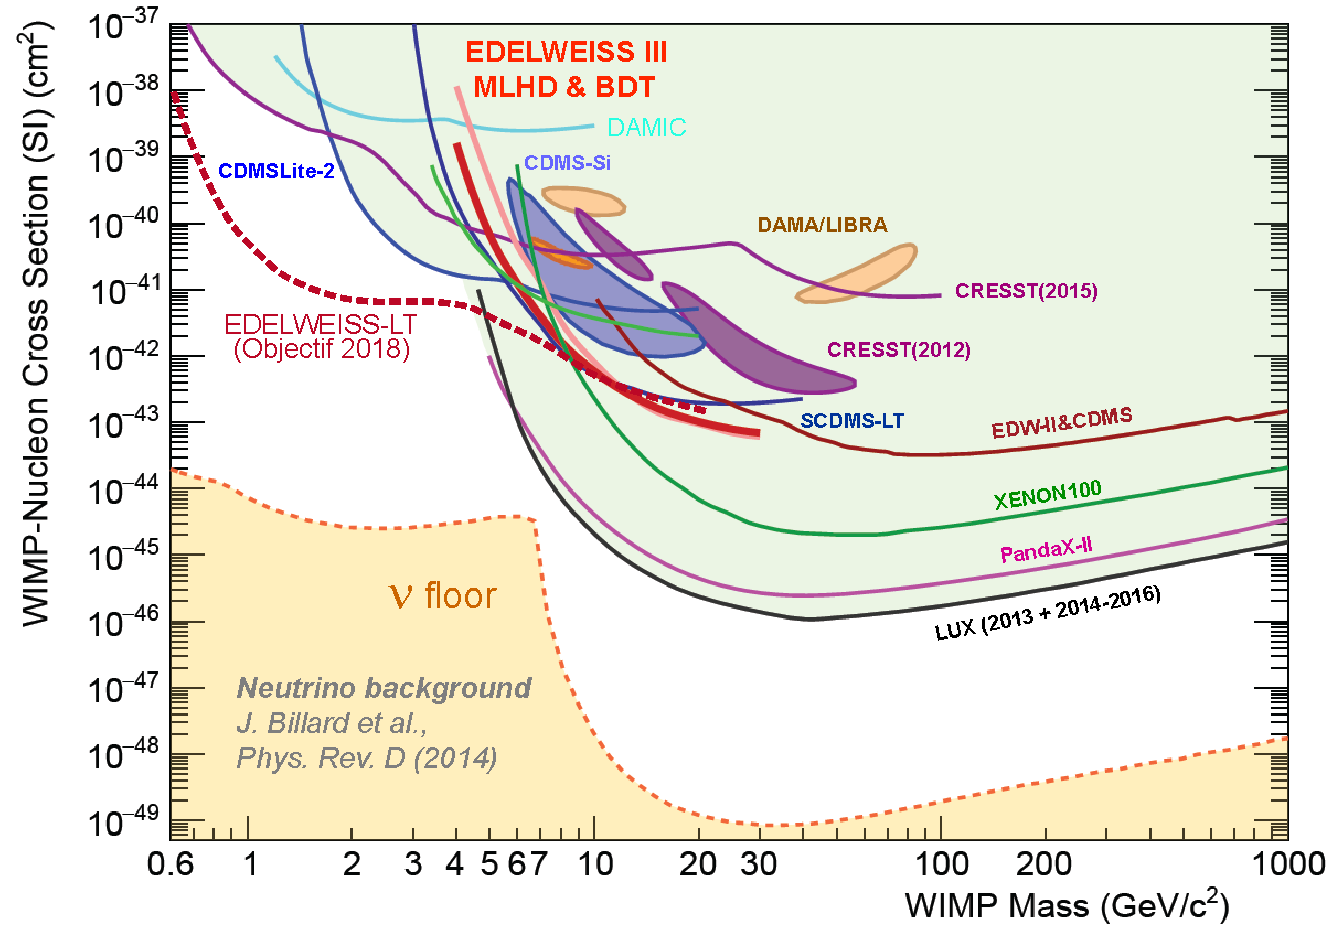
\includegraphics[width=0.75\textwidth]{Images/stateofart.pdf}
%\end{center}
%\caption[]{
%Diagramme de l'état de l'art pour la détection directe de WIMP. Dans l'espace de masse du WIMP et de la section efficace d'interaction WIMP-nucléon, il est représenté :
%%\begin{itemize}
%%\item en traits pleins : les courbes d'exclusions, chacune associée à une expérience de détection,
%%\item en bleu : l'espace déjà sondé et exclu,
%%\item en blanc : l'espace restant à être sondé,
%%\item en orange : limite de détection directe fixée par les neutrinos cosmiques,
%%\item les contours colorés : détections possibles de WIMPs, cependant exclues par d'autres résultats négatifs,
%%\item courbe rouge pointillée : objectif de la collaboration EDELWEISS pour 2018.
%%\end{itemize}
%}
%\label{art}
%\end{figure}
%\section*{Introduction}
%
%
%This diagram allows to visualize the exclusion curves drawn by the different collaborations, the space already surveyed, the intrinsic limit to direct detection set by cosmic neutrinos, and the space still to be surveyed. The latter is divided into two zones. The first concerns high mass WIMPs ($>10 GeV$) which deliver high recoil energy at the cost of a very low interaction cross section. Probing this area requires very massive detectors that can accumulate large exposures. The second area concerns low mass WIMPs ($<10 GeV$): this is the research area of EDELWEISS. The effective cross section is higher, so there is less concern about exposure. Nevertheless, the mass being small, the deposited recoil energy is also low. It is therefore necessary to work with detectors whose energy detection threshold is sufficiently small. The objective of the EDELWEISS collaboration for the year 2018 is a new exclusion curve (drawn in red dashes on the figure \ref{art}) requiring the development of a detector fulfilling the "$4\times 100$" objective described below.
%
%\subsection{The EDELWEISS experiment and the $4\times 100$} objective
%
%The name EDELWEISS stands for Experience for Detecting Underground WIMPs.
%This experiment uses cryogenic detectors in a cryostat that allows the temperature to drop down to $18mK$ and a very high vacuum. Direct detection with low energy detection threshold requires to reduce to the maximum any source of noise. 
%
%This is why the cryostat containing the detectors is placed within a shielding of layers of lead (including archaeological lead) and polyethylene to reduce as much as possible the impact of gamma radiation from the ambient radioactivity and the surrounding neutron background, respectively. This shielding is itself surrounded by a muon detection device called a "muon veto" which allows active discrimination of muons because they can produce neutrons in the detector enclosure. Finally, the EDELWEISS experiment is carried out in the Modane Underground Laboratory, in the middle of the Fréjus Tunnel, sheltered by more than $1700$m of rock. This natural barrier reduces the flow of cosmic muons by a factor of 6, which gives favorable conditions for direct detection with low energy thresholds.
%
%The detectors used by the EDELWEISS collaboration aim to measure the recoil energy deposited as ionization and heat. The objective 2018 to obtain a new exclusion curve requires the development of a new generation of detectors. The energy detection threshold must be increased from $2$keV to $100$eV. To do this, the objective "$4\times 100$" must be met:
%\begin{itemize}
%\item 100 Volts of voltage applied to the absorber. The charges created by ionization contribute to increase the heat signal by the Luke effect by drifting towards the collection electrodes. Increasing the voltage is equivalent to amplifying the heat signal.
%\item 100 eV resolution in ionization. 
%\A 100-fold decrease in heat-only events. These are non-ionizing background noise events that prevent the detection of a potential WIMP signal.
%\item 100 eV resolution in heat channel.
%\end{itemize}
%The first three points have been obtained or are in the process of being obtained. Only the improvement of the heat path remains necessary to meet the "$4\times 100$" objective and thus draw a new exclusion curve. 
%
%My internship work is part of the EDELWEISS R\&D campaign to improve the energy resolution of the heat channel of its detectors. A series of simplified "RED" detectors has been created for this purpose.
%The objective of my internship is to study the designs of the detectors, to build a complete thermal model of the detectors, to characterize the electronic noise of the detectors and finally to start the optimization process.

